\chapter{Introducción}
\label{cap:capitulo1}
\setcounter{page}{1}
\pagestyle{plain}

La tarea Sigue-Personas es una de las más empleadas y solicitadas en los Robots de Servicio para multitud de sectores que incorporan soluciones robóticas. El siguiente TFG propone desarrollar dos nuevos ejercicios para Robotics Academy con el fin de que sean integrados en la plataforma Unibotics, con el objetivo de que los usuarios programen un robot Turtlebot2 tanto simulado como real para que realice dicha tarea.\\

Este primer capítulo trata de presentar el estado actual de varios campos de la Robótica que están directamente relacionados con este proyecto para poner en contexto al lector y facilitar su lectura.\\

Por un lado presentaremos la Robótica Móvil, un sector de la robótica que está en constante crecimiento y muy presente en la Robótica de Servicio; por otra parte, introduciremos las Redes Neuronales, un avance significativo en IA que ha permitido realizar aplicaciones muy robustas basadas en la percepción y el razonamiento; y por último hablaremos de la Robótica Educativa, e introduciremos varias plataformas como TheConstruct, Robotics Academy, o Unibotics siendo estas dos últimas las que incorporarán el ejercicio educativo Sigue-Persona.




% -- ROBOTICA MOVIL
% -------------------
\section{Robótica Móvil}
\label{sec:robotica_movil}

La robótica es la ciencia que engloba varias ramas tecnológicas o disciplinas, con el objetivo de diseñar máquinas (``robots'') que sean capaces de realizar tareas automatizadas o de simular el comportamiento humano o animal, en función de la capacidad de su software. \cite{revistaderobots}. Su término se remonta a la obra de ciencia ficción escrita por Isaac Asimov: Yo, Robot. (1950)\\

Una vez que la robótica emerge a partir de mediados del siglo XX, surgen 2 sectores: la Robótica Industrial y la Robótica de Servicio. Los \textit{Robots industriales} se encargan de realizar tareas automatizadas y muy repetitivas en escenarios industriales, donde el entorno está muy controlado. Los \textit{robots de Servicio} son aquellos que realizan tareas útiles para el ser humano y mejorar su comodidad. Entre los robots de servicio, destacan los robots móviles.\\

Un \textit{robot móvil} es un sistema electromecánico capaz de desplazarse de ma­nera autónoma sin estar sujeto físicamente a un solo punto\cite{robots-moviles-evolucion-estado-arte}. Posee sensores que permiten monitorear en cada momento su posición relativa a su punto de origen (odometría) y a su punto de destino. Normalmente su control se basa en un sistema de lazo cerrado (modo de actuación está determinado por su estado anterior). Se clasifican en robots móviles de locomoción con \textit{ruedas}, locomoción con \textit{patas} y locomoción con \textit{orugas}.  Los primeros son más fáciles de controlar pero no se adaptan bien a muchas superficies, sin embargo los robots con patas (cuadrúpedos o bípedos) se adaptan muy bien a distintas superficies pero requieren varios controladores para mantener su equilibrio tanto estático como dinámico. El entorno en el que se enfrentan es bastante \textit{heterogéneo}, por tanto su software debe ser lo más robusto posible para adaptarse correctamente a los cambios.\\




% -- EVOLUCION HISTORICA
% ------------------------
\subsection{Evolución Histórica}
\label{subsec:evolucion_historica}

Podemos destacar varios hechos importantes a lo largo del siglo XX y principios del XXI que 
marcaron grandes avances en la robótica:

\begin {itemize}
	\item En 1952 aparece la primera máquina de control numérico del MIT que era capaz de automatizar algunas tareas industriales.
	\item En 1961, la compañía Unimates introdujo el primer robot industral en la General Motors.
	\item En 1966, comenzó el desarrollo del primer robot móvil llamado Shakey [Nilsson, 1984]
	\begin{figure} [H]
	\begin{center}
	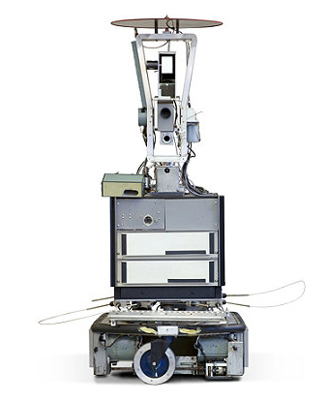
\includegraphics[width=5cm]{imagenes/shakey.jpg}
	\end{center}
	\caption[Shakey (1966-1972)]{Shakey (1966-1972) Imagen obtenida de \cite{shakey-the-robot}.}
	\label{fig:shakey}
	\end{figure}\
	\item En los años 70, NASA desarrolló MARS-ROVER, una plataforma móvil que integraba un brazo mecánico, sensores de proximidad, un dispositivo telemétrico láser y cámaras estéreo
	\item En 1997, la NASA envió a Marte un dispositivo móvil llamado Sojourner Rover, para enviar fotografías a la Tierra del planeta rojo. Además, la empresa HONDA sacó el primer humanoide capaz de imitar comportamientos humanos
	\item En 2000, Honda presenta el robot Asimo.
	\item En 2004, Qrio de Sony, un pequeño robot humanoide capaz de correr, bailar, y reconocer caras.
	\item En 2008, SoftBank Robotics presenta el Robot \textit{Nao}, un robot bípedo dedicado a interactuar con el ser humano y ser muy amigable. En 2014, la empresa presenta el robot \textit{Pepper}, robot con forma humana pero se desplaza con ruedas. Se ha usado sobre todo como robot guía, recepcionista y en exhibiciones, sin embargo, fue abandonado en 2021 (Figura \ref{fig:nao_pepper})
	\begin{figure} [H]
		\begin{center}
		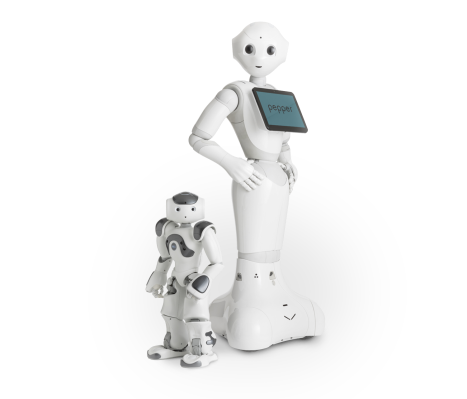
\includegraphics[width=10cm]{imagenes/cap1/nao-pepper.png}
		\end{center}
		\caption[Nao y Pepper]{Nao y Pepper. Imagen obtenida de \cite{softbank-robotics}.}
		\label{fig:nao_pepper}
	\end{figure}
	\item En 2013, Boston Dynamics saca a la luz el robot \textit{Atlas}, un humanoide con actuadores neumáticos. La empresa lo usa para imitar el comportamiento humano llevándolo a otro nivel haciendo acrobacias o incluso parkour. En 2020, la empresa saca a la venta un robot cuadrúpedo llamado \textit{Spot} que imita el comportamiento de un perro, que se usa en algunas fábricas para transportar materiales o realizar tareas de mantenimiento (Figura \ref{fig:atlas_spot})
	
	\begin{figure} [H]
		\begin{center}
		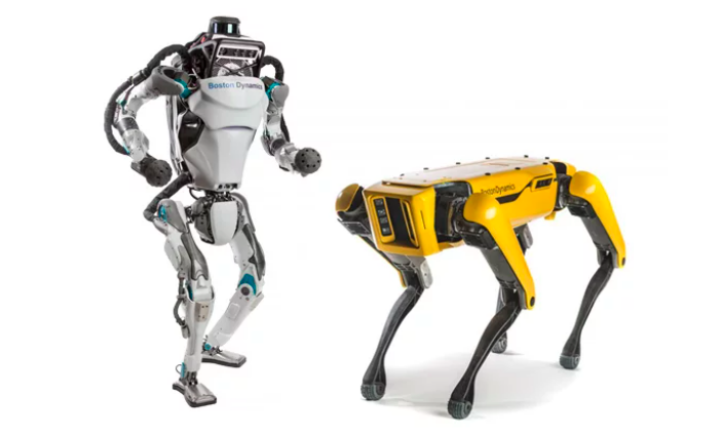
\includegraphics[width=10cm]{imagenes/cap1/spot-atlas.png}
		\end{center}
		\caption[Atlas y Spot]{Atlas y Spot. Imagen obtenida de \cite{spot-atlas}.}
		\label{fig:atlas_spot}
	\end{figure}\
\end{itemize}



% -- APLICACIONES ACTUALES
% --------------------------
\subsection{Aplicaciones actuales}
\label{subsec:aplicaciones_actuales}
Como hemos visto, el avance de los robots móviles ha emergido durantes estas últimas décadas. Con ellos han surgido una gran diversidad de aplicaciones:

\begin{enumerate}
	\item Aplicaciones domésticas. Podemos destacar los robots de limpieza como \textit{Roomba} (robot aspirador) y \textit{Braava} de iRobot (robot friegasuelos) o \textit{WinBot} de Ecovacs (limpia ventans). La realización de sus tareas se logra mediante algoritmos de navegación y cobertura para limpiar el mayor espacio en el menor tiempo posible.
	\item Agricultura. Incorporación de tractores o vehículos autónomos encargados del mantenimiento y monitorización de los cultivos.
	\item Inspección y mantenimiento en zonas críticas (centrales nucleares) o poco seguras para el ser humano
	\item Reparto. Muy empleado en la logística, o como prototipo para las entregas a domicilio (última milla).
	\item Enseñanza. Robots móviles usados en las ingenierías como el robot Turtlebot2 (robot usado en este proyecto).
\end{enumerate}\



% -- MACHINE LEARNING
% ---------------------
\section{Machine Learning}
\label{sec:machine_learning}
La \textit{Inteligencia Artificial} (IA) es un campo muy extenso que está evolucionado rápidamente en este siglo XXI. Se basa en el estudio de algoritmos que permitan a las máquinas realizar tareas de manera ``inteligente'' (búsqueda, lógica, teoría de juegos, planificación). Sin embargo, la IA es sólo una \textit{apariencia}. Cuando incorporamos a un computador la capacidad de \textit{aprendizaje} es entonces cuando hablamos de \textit{Machine Learning}\\

Según \emph{Arthur Samuel}, el \textit{Aprendizaje Automático} o \textit{Machine Learning} es el ``campo de estudio que otorga a los ordenadores la capacidad de aprender sin ser programados explícitamente''. Para ello se emplean diversas técnicas dependiendo del resultado deseado: Regresión Lineal, Regresión Logística, K-NN, K-Means, SVM, Redes Neuronales, Q-Learning, etc.\\


\section{Redes Neuronales Artificiales (RNA)}
\label{sec:redes_neuronales}

Una \textit{Red Nueronal Artificial (RNA)} es un modelo computacional inspirado en el cerebro humano que sirve para \textit{clasificar} datos de entrada con su correspondiente salida a partir de un entrenamiento previo. Para ello se le proporciona un \textit{dataset} (conjunto de datos), donde indicamos, por cada muestra, a qué clase pertenece (Aprendizaje Supervisado). Al iniciar el entrenamiento, se realiza un proceso de optimización ajustando los valores de unas variables que actúan como pesos o cargas de las \textit{dendritas} de las \textit{neuronas}, consiguiendo un nivel de clasificación determinado. Pero, ¿cómo funciona una neurona?\\

Una neurona, tal y como se muestra en la figura \ref{fig:neurona} está formada pos los siguientes elementos:
\begin{itemize}
	\item \textbf{Valores de Entrada}: Puede ser tanto los valores de las \textit{características} de cada muestra como la salida de la neurona de una capa anterior.
	\item \textbf{Pesos}: Son unos valores que se optienen al final de la etapa de entrenamiento.
	\item \textbf{Sumatorio}: Esta formado por los productos de los Valores de Entrada por sus correspondientes Pesos
	\item \textbf{Función de Decisión/Activación}: Es una función matemática que se aplica al sumatorio: Lineal, Escalón, Sigmoide, etc
	\item \textbf{Salida}: Es el valor de la función de decisión. Dependiendo de la función de activación usada, la salida será distinta.
\end{itemize}

\begin{figure}[H]
  \begin{center}
    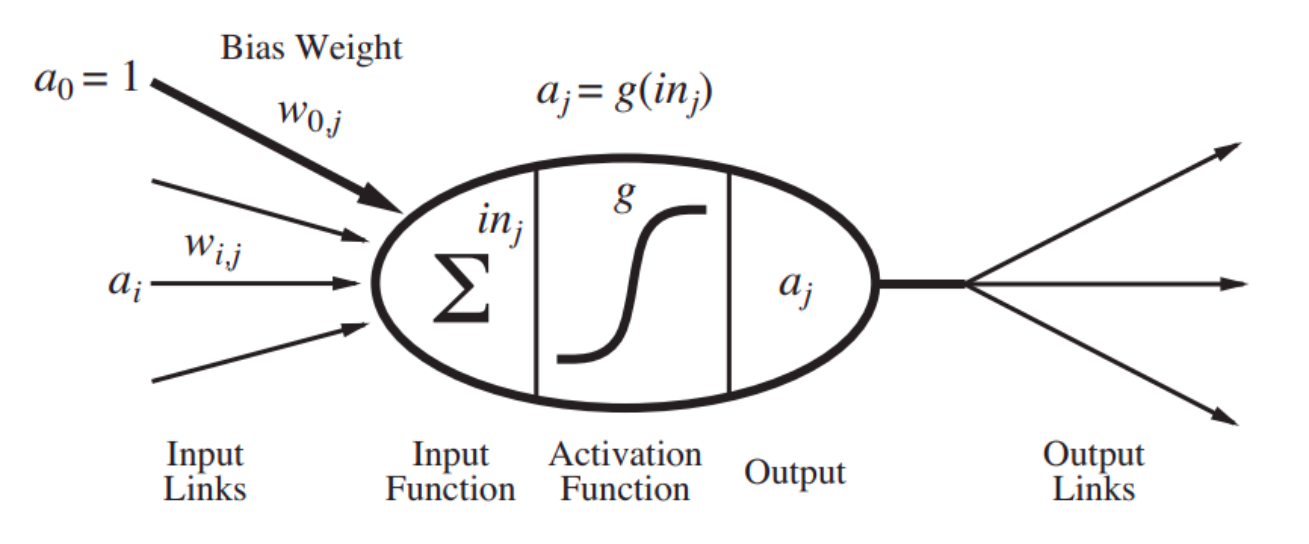
\includegraphics[width=15cm]{imagenes/neurona.png}
  \end{center}
  \caption[Modelo computacional de una neurona]{Modelo computacional de una neurona \cite{AIMA}}
  \label{fig:neurona}
\end{figure}

Tomando como ejemplo un perceptrón (neurona utilizada para resolver tareas de clasificación binaria) la clasificación se realiza mediante un \textit{hiperplano de separación} sujeto a la función de decisión (función escalón) separando en dos clases (0 o 1) los datos de entrada. La posición y orientación del hiperplano de separación está determinado por el proceso de optimización realizado durante el entrenamiento de la neurona. En la siguiente Figura mostramos dos ejemplo de un perceptrón entrenado a partir de cuatro datos de entrada que simulan una puerta lógica AND y OR respectivamente:\\

\begin{figure}[H]
  \begin{center}
    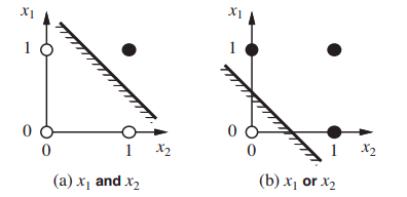
\includegraphics[width=10cm]{imagenes/cap1/ejemplo-perceptron.png}
  \end{center}
  \caption[Salida de un perceptrón de tipo AND y OR]{Salida de un perceptrón de tipo AND y OR \cite{AIMA}}
  \label{fig:salida_perceptron}
\end{figure}\

Cuando los datos de entrada no son linealmente separables mediante un hiperplano de separación es cuando necesitamos aumentar el número de neuronas. Normalmente, una RNA consta de un conjunto de capas formado por varias neuronas que se encuentran interconectadas. Suelen dividirse en 1 capa de entrada, 1 o más capas ocultas y 1 capa de salida.\\

Cuando el problema de clasificación involucra una gran cantidad de información y entradas como puede ser un video o una imagen, se usan modelos de redes neuronales profundas (\textit{Deep Neural Networks}, DNN) de varias capas con un elevado número de neuronas. Variante de \textit{Machine Learning} conocida como \textit{Deep Learning}\\

\begin{figure}[H]
  \begin{center}
    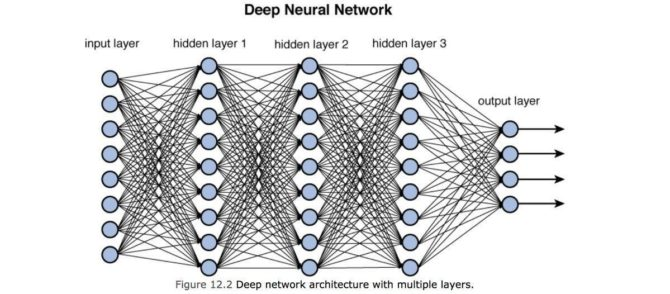
\includegraphics[width=15cm]{imagenes/cap1/dnn.jpeg}
  \end{center}
  \caption[Red Neuronal Profunda (DNN)]{Red Neuronal Profunda. Imagen obtenida de \cite{dnn}}
  \label{fig:salida_perceptron}
\end{figure}\

Una aplicación muy popular de Redes Neuronales es la detección de objetos mediante \textit{Vision Artificial}: dada una imagen/fotograma como valor de entrada, la red neuronal es capaz de detectar ciertos objetos solicitados como puede ser fruta, coches, utensilios o incluso personas y animales dependiendo del entrenamiento aplicado.\\


\subsection{Redes Neuronales Convolucionales (CNN)}
\label{subsec:redes_convolucionales}

Las \textit{Redes Neuronales Convolucionales, CNN} son un tipo de RNA multicapa aplicados para identificar y \textit{clasificar} objetos en una imagen o video. Se basan en la \textit{Convolución de capas}. El funcionamiento de la convolución trata de iterar sobre todos los píxeles de una imagen y aplicar varios filtros de \textit{Kernel} \footnote{\textbf{Filtro Kernel}: En Vision Artificial, es una matriz cuadrada a la que se le aplica un producto escalar a una región de píxeles con la misma dimensión} obteniendo así varias matrices de píxeles, las cuales se les aplican una función de \textit{decisión} obteniendo una mapa de detección de características.\\

La siguiente capa tendrá matrices más pequeñas debido a la reducción de los mapas de características (\textit{Max-Polling}), y así sucesivamente, hasta que en las últimas capas obtenemos patrones que diferencian a unos objetos de otros. A la última capa oculta de neuronas se le aplica una función llamada \textit{Softmax} generando una capa de salida con el mismo número de neuronas que de clases.\\

Al usar la CNN dada una imagen obtendremos una lista de porcentajes normalizados de 0 a 1 indicando el grado de probabilidad de que la imagen se corresponda con cada clase. En la siguiente Figura [\ref{fig:ocr_cnn}] podemos ver un ejemplo de OCR (Reconocimiento Óptimo de Caracteres) usando CNN.\\

\begin{figure}[H]
  \begin{center}
    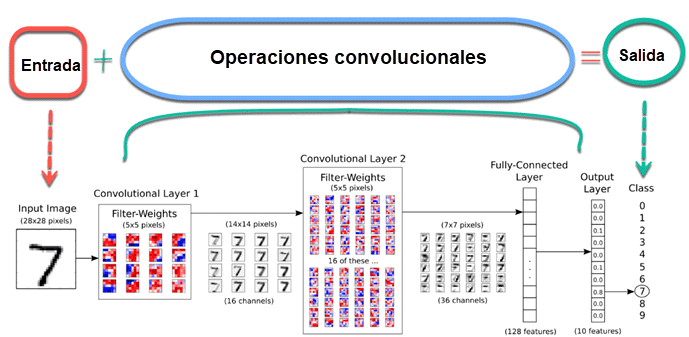
\includegraphics[width=15cm]{imagenes/cap1/ocr-cnn.png}
  \end{center}
  \caption[OCR usando CNN)]{OCR usando CNN. Imagen obtenida de \cite{dnn}}
  \label{fig:ocr_cnn}
\end{figure}\

A partir de CNN surge otro tipo de RNA, denominado R-CNN (\textit{Region-based Convolutional Neural Network}) que permite \textit{detectar} varios objetos en una imagen y que utilizaremos en este proyecto para realizar la tarea de seguir a una persona. Su funcionamiento se basa en la extracción de regiones de interés que pasan a través de una CNN devolviendo el resultado de una clasificación. Las regiones que pintamos según el resultado de la CNN se conocen como \textit{Bounding Boxes}.

\begin{figure}[H]
  \begin{center}
    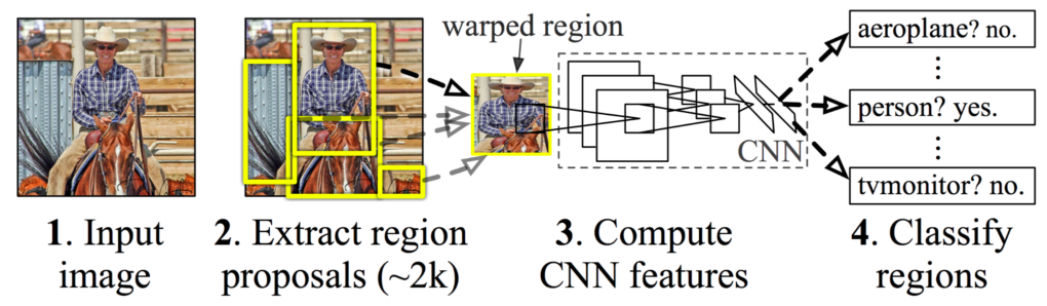
\includegraphics[width=15cm]{imagenes/cap1/r-cnn.png}
  \end{center}
  \caption[Ejemplo de R-CNN]{R-CNN. Imagen obtenida de \cite{r-cnn}}
  \label{fig:r-cnn}
\end{figure}\

Actualmente, hay disponibles varias arquitecturas de R-CNN para implementar aplicaciones de Machine Learning basada en la detección de objetos:

\begin{itemize}
	\item \textbf{YOLO} (You Only Look Once)
	\item \textbf{SSD Inception}
\end{itemize}


\section{Educación en Robótica}
\label{sec:educacion_robotica}

\subsection{Grado en Ingeniería de Robótica Software (URJC, España)}
\label{subsec:grado_robotica_software}
La Universidad Rey Juan Carlos (España) imparte en el campus de Fuenlabrada, el grado en Ingeniería de Robótica Software (primer año: 2018) para enseñar a los futuros ingenieros interesados en este campo a programar la \textit{inteligencia} de los robots del futuro.\\

Tal y como indica el título del grado, se trata de una carrera universitaria de programación, donde los alumnos abarcarán varios temas como por ejmplo Inteligencia Artificial, visión artificial, programación de lenguajes de alto nivel (C++, Python...), Seguridad, Drones, robots de servicio, robótica industrial, y mucho más. Las clases se imparten tanto en salas de ordenadores con sistemas operativos Linux (distribución Ubuntu) como en el laboratorio de Robótica, donde los alumnos podrán programar directamente robots reales.\\

El robot usado en este Trabajo Fin de Grado es un modelo Turtlebot 2 de Yujin. Consta de una base (kobuki) similar a la de un robot de limpieza con sensores de contaco (bumpers), y un soporte encima que le permite incorporar un RPLIDAR, una cámara, y colocar el portátil del estudiante cuando desarrolla una solución al problema.

\subsection{The Construct}
\label{sec:the_construct}
The Construct es una organización que mantiene una plataforma para aprender robótica con ROS, un framework para programar robots muy utilizado en este sector. Imparten varios cursos donde los usuarios acceden a máquinas virtuales con un Linux instalado y todas las dependencias adquiridas.\\

\begin{figure}[H]
  \begin{center}
    
\includegraphics[width=10cm]{imagenes/cap1/the-construct.png}
  \end{center}
  \caption[Plataforma web de The Construct]{Plataforma web de The Construct\cite{the-construct}}
  \label{fig:r-cnn}
\end{figure}\

\subsection{Robotics Academy}
\label{sec:robotics_academy}
Robotics Academy \cite{robotics-academy} es una colección de ejercicios y desafíos para aprender robótica. Está mantenido por la organización JdeRobot. Sus ejercicios abarcan varios temas: drones, robótica móvil, visión artificial, coches autónomos, robótica industrial, etc. Además es una plataforma Open Source, por lo que cualquier interesado/a puede contribuir desde Github.\\

En sus orígenes, solo se podía ejecutar sobre un sistema operativo Linux, pero desde sus últimas versiones puede ejecutar también sobre Windows y MAC, gracias a la incorporación de plantillas web que se ejecutan en un navegador estableciendo una conexión a través de WebSockets con un contenedor software (Docker) que lanza el usuario, permitiendo de esta manera, el despliegue de los ejercicios sobre un sistema operativo virtualizado y con todas sus dependencias ya instaladas.\\

Los usuarios una vez que escogen un ejercicio y lanzan el contenedor obtienen acceso a una dirección web local donde pueden empezar a programar. La plantilla web incorpora un Editor de Texto y la posibilidad de visualizar un simulador y un terminal mediante una conexión VNC con el contenedor. En la figura \ref{fig:rob-ac-web-template} vemos un ejemplo de plantilla web correspondiente al ejercicio \textit{Follow Person}. La programación se realiza con Python (un lenguaje fácil de entender y aprender, y muy usado en la Robótica).\\

\begin{figure} [h!]
  \begin{center}
    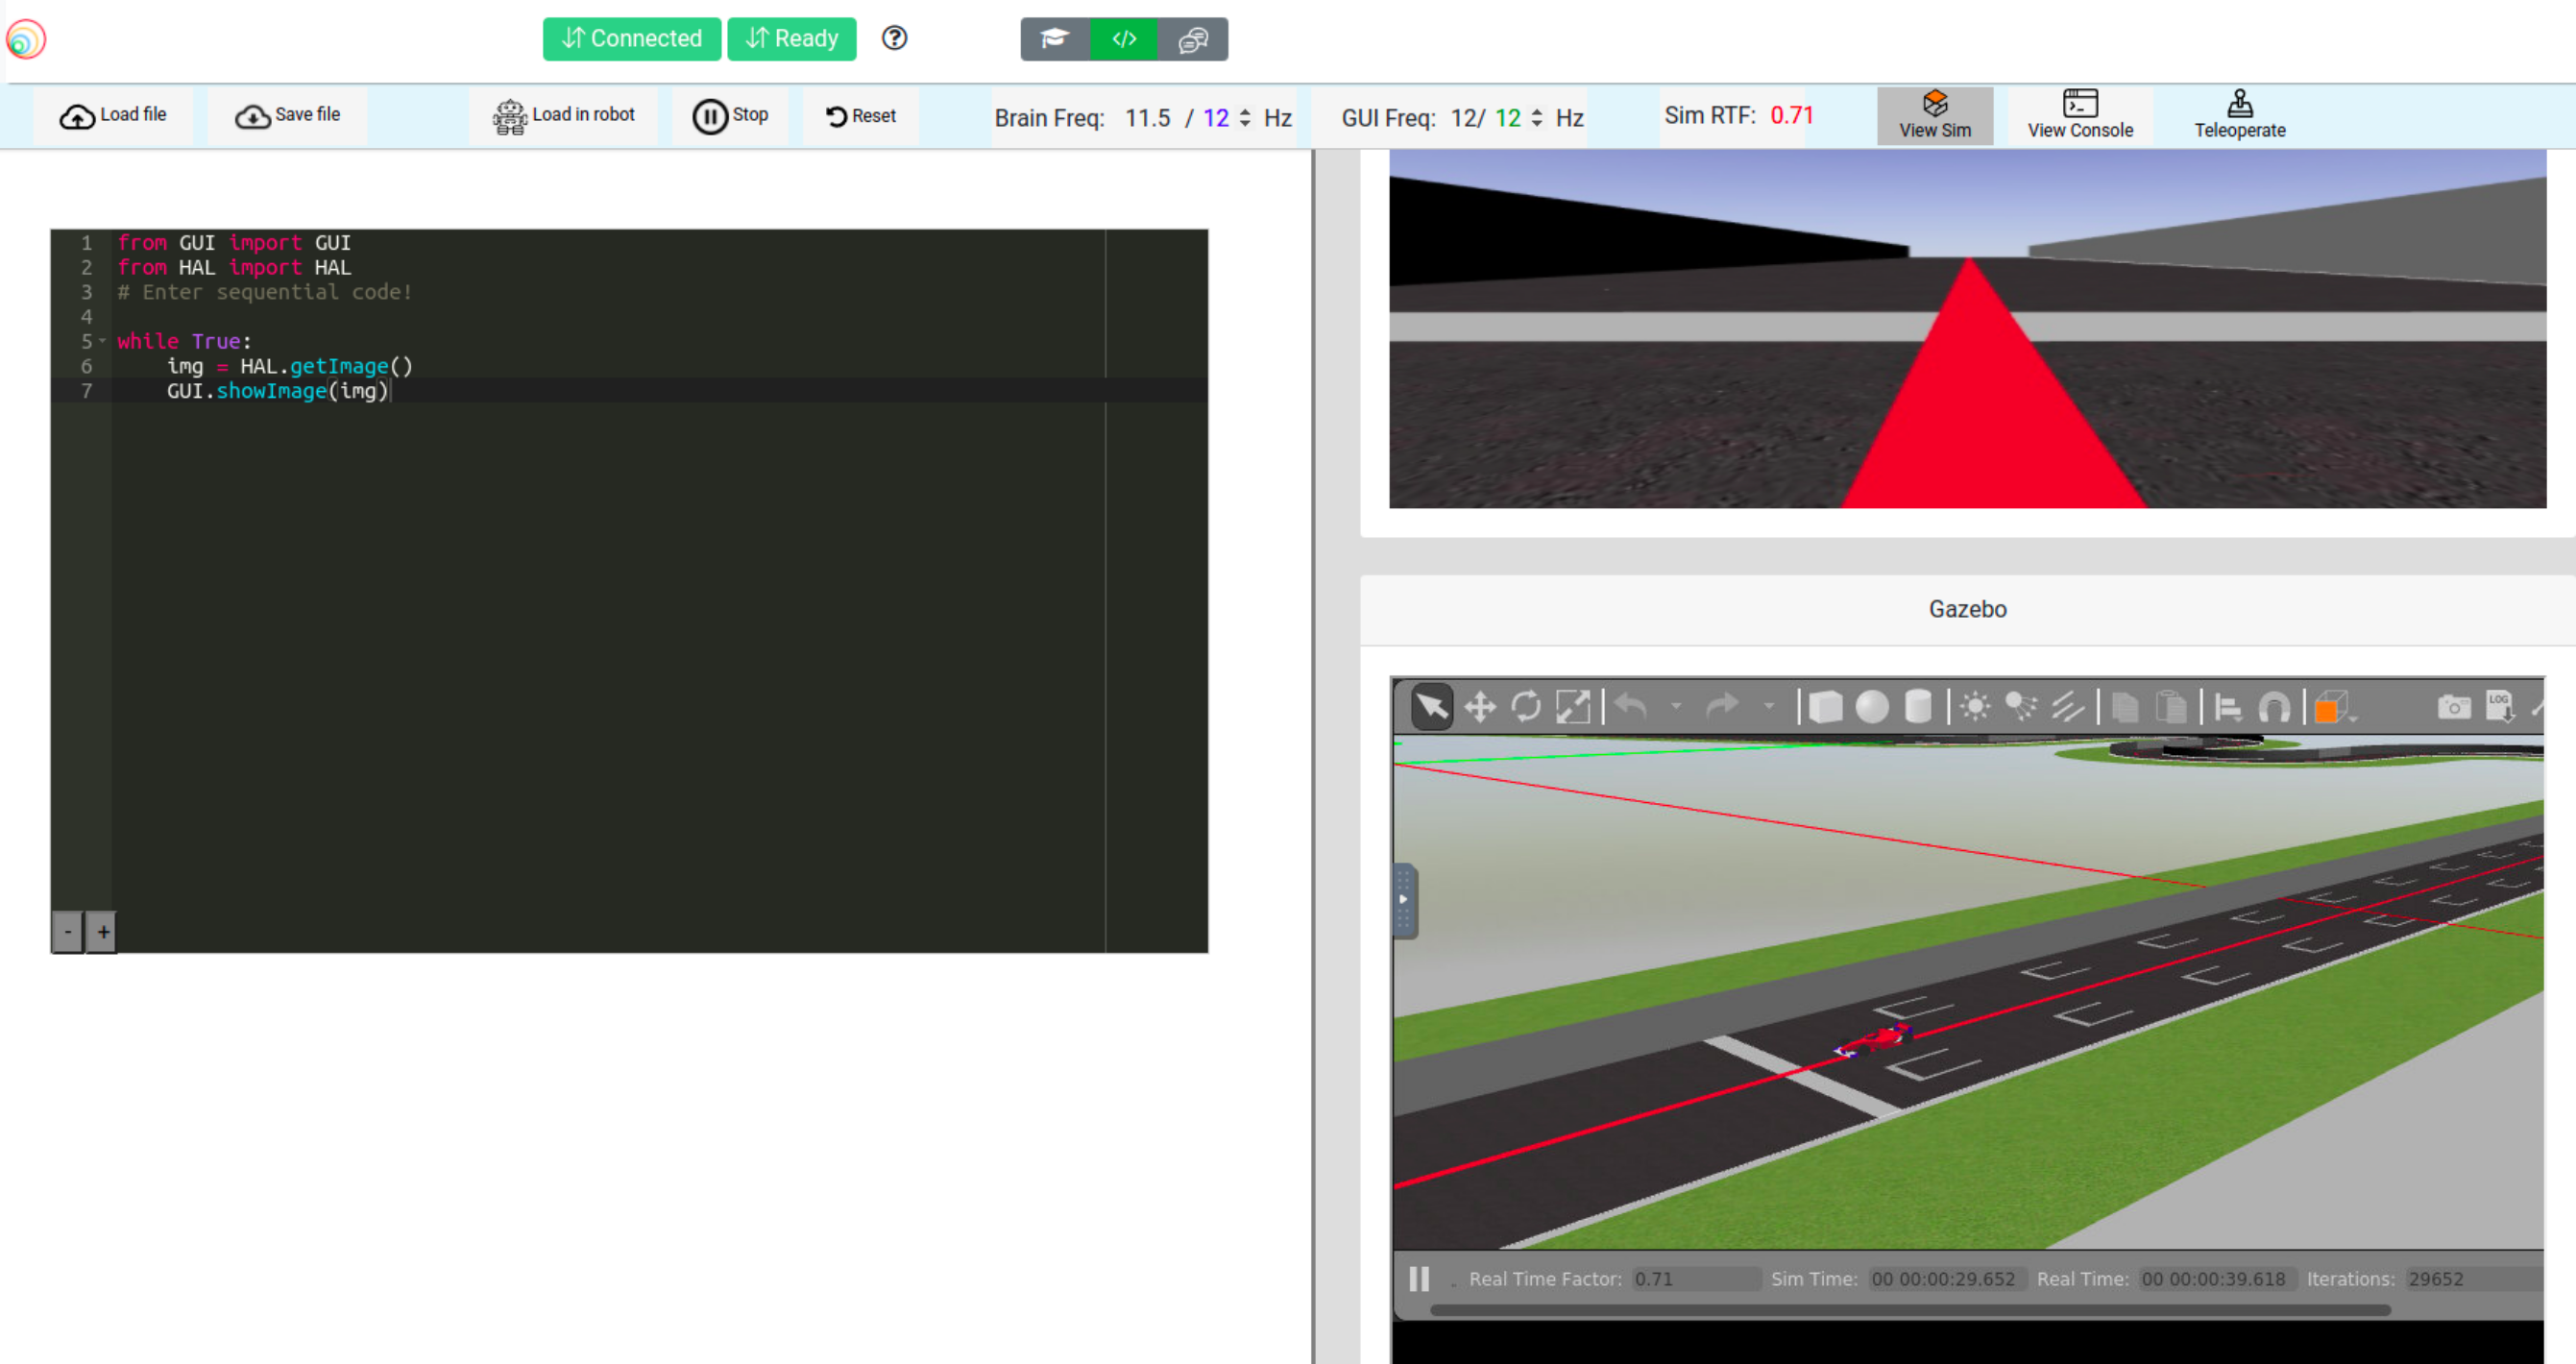
\includegraphics[width=10cm]{imagenes/cap1/robotics-academy-web-template.png}
  \end{center}
  \caption[Robotics Academy (Web Template)]{Robotics Academy (Web Template)}
  \label{fig:rob-ac-web-template}
\end{figure}\

Una ventaja de usar Robotics Academy, es que permite al usario centrarse única y exclusivamente en el algoritmo que tiene que implementar. Toda la complejidad relacionada con la comunicación con el hardware del robot: motores, laser, cámara, etc. que, por lo general se realiza mediante ROS (un framework para programar Robots) queda encapsulado por 2 módulos de Python: HAL y GUI. De esta manera, el usuario dispone de una API de HAL (Hardware Abstración Layer) para comandar a los actuadores o recibir información de los sensores, y una API de GUI (Graphical User Interface) para visualizar por el navegador información como puede ser una imagen, un mapa o incluso vectores.\\

\subsection{Unibotics}
\label{sec:unibotics}

\textbf{Unibotics} es una plataforma de Robótica que incorpora parte de la coleción de ejercicios de Robotics Academy. Con Unibotics, JdeRobot da un nuevo paso, permitiendo a los usuarios registrarse en un servidor donde pueden guardar sus códigos, acceder cuando deseen, y, poder contar con la posibilidad de lanzar los ejercicios en un servidor remoto proporcionando la opción de no instalar un contenedor software en sus sistemas operativos.\\

Una vez que el usuario introduce sus credenciales y accede a su sesión, tiene una lista de ejercicios disponibles [Figura \ref{fig:menu-unibotics}], que funcionan de la misma manera que aquellos que proporciona \textit{Robotics Academy}. Actualmente todos los ejercicios disponibles están implementados usando dentro del sistema operativo virtual la distribución ROS Noetic como base.\\

Con los 2 nuevos ejercicios Sigue-Personas que explicaremos en este proyecto, pretendemos integrarlos en Unibotics usando ROS Foxy como base. De esta manera, marcaremos un inicio para la migración de varios ejercicios de ROS Noetic a ROS Foxy.\\

\begin{figure} [H]
  \begin{center}
    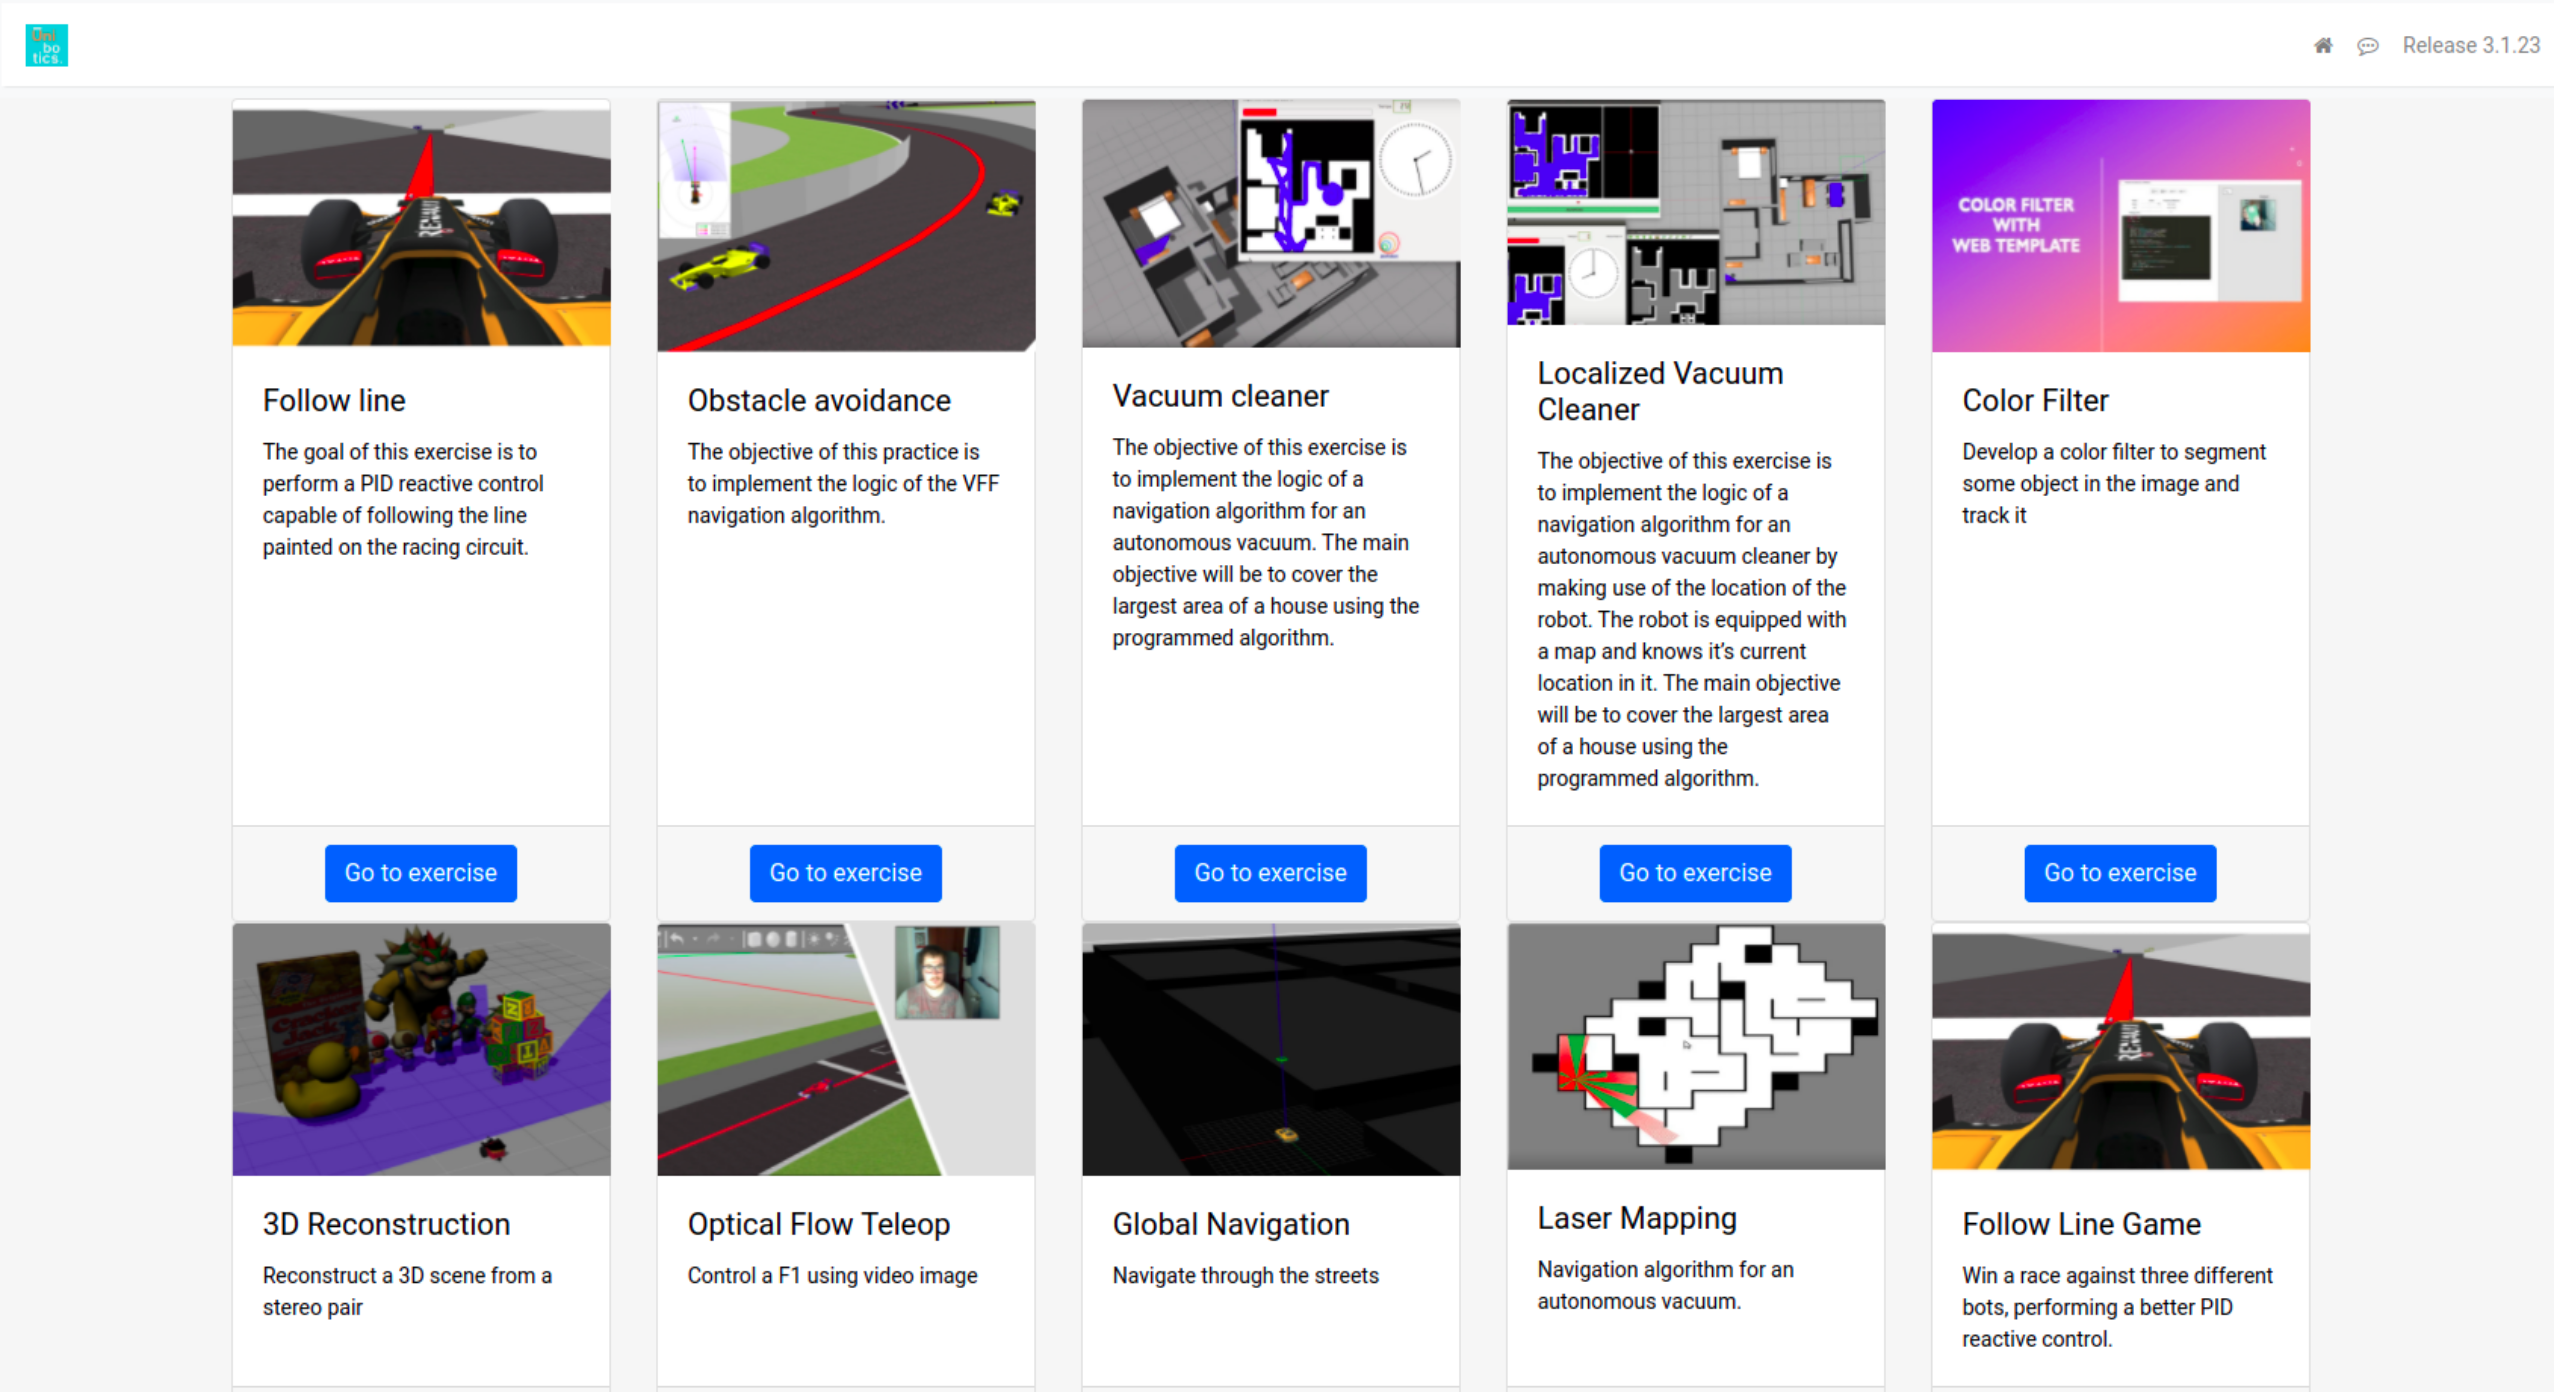
\includegraphics[width=10cm]{imagenes/cap1/unibotics-menu.png}
  \end{center}
  \caption[Unibotics (Menú)]{Unibotics (Menú)}
  \label{fig:menu-unibotics}
\end{figure}




